\section{Lampknappar}
Vi börjar med att göra ett par observationer:
\begin{enumerate}
  \item Det finns ingen anledning att släcka lampor tidigt, utan man kan vänta till slutet med att göra det.
    Givet en lösning det att göra om det till en som väntar till slutet på följande sätt:
    \begin{itemize}
      \item simulera lösningen, men ignorera alla lampsläckningar
      \item gå motsatta vägen tillbaka till starten
      \item simulera lösningen igen, men släck nu varje rums lampa när du går ut ur rummet för sista gången
    \end{itemize}
    Eftersom varje lampa är tänd minst lika länge i den sista simuleringsprocessen kommer denna lösning fungera om den ursprungliga gör det,
    och vi noterar att vi först tänder alla lampor, och sen släcker dem.
  \item Problemet är symmetriskt: en lösning som går från rum $1$ till rum $N$ kan reverseras för att få en lösning som går från rum $N$ till rum $1$.
    En följd av detta är att rummen vi lyser upp i vår lösning kommer innehålla både en väg från nod $1$ till nod $N$, och en väg från nod $N$ till nod $1$.
  \item Det räcker att bara lysa upp dessa rum. Givet en väg från nod $1$ till nod $N$ och en väg från nod $N$ till nod $1$ kan vi göra följande:
    \begin{itemize}
      \item Gå från rum $1$ till rum $N$ och lys upp allt på vägen.
      \item Gå från rum $N$ till rum $1$ och lys upp allt på vägen.
      \item Gå från rum $1$ till rum $N$ igen.
      \item Ångra vandringen från rum $1$ till $N$ genom att gå motsatta hållet.
        När vi för sista gången går ut ur ett rum som inte är med i vandringen från rum $N$ till rum $1$, släck lampan i rummet.
      \item Ångra vandringen från rum $N$ till $1$ genom att gå motsatta hållet.
        När vi för sista gången går ut ur ett rum, släck lampan i rummet.
    \end{itemize}
    Det som får det här att funka är att vi alltid kan ångra en vandring genom att gå åt motsatt håll, utan att nånsin fastna i ett mörkt rum.
\end{enumerate}

\begin{figure}[!h]
\begin{center}
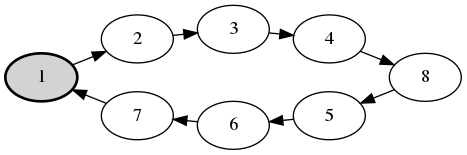
\includegraphics[width=5cm]{astep1.png}
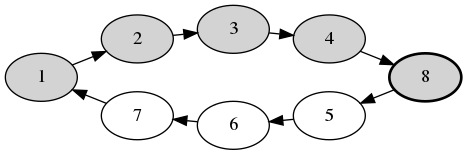
\includegraphics[width=5cm]{astep2.png}
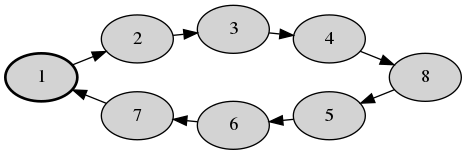
\includegraphics[width=5cm]{astep3.png}
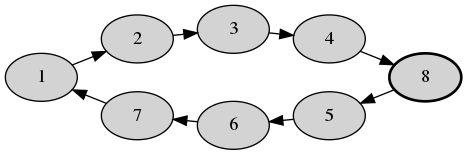
\includegraphics[width=5cm]{astep4.png}
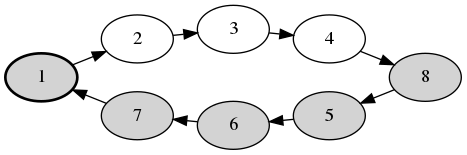
\includegraphics[width=5cm]{astep5.png}
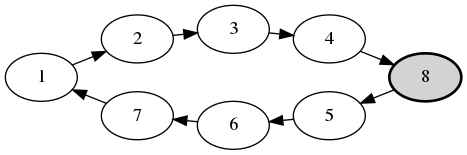
\includegraphics[width=5cm]{astep6.png}
  \caption{Illustration över hur lampornas tändande och släckande kan gå till, givet en väg från första till sista noden, och en väg från sista till första. Vägarna överlappar i det här fallet inte. En ifylld ruta betecknar ett upplyst rum, och tjock ram betyder att Ann just nu befinner sig i det rummet. Stegen visas vänster till höger, uppifrån ner.}
\end{center}
\end{figure}

\begin{figure}[!h]
\begin{center}
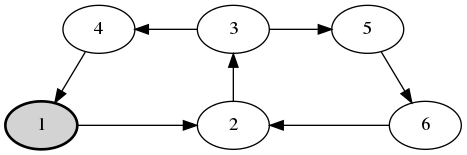
\includegraphics[width=5cm]{bstep1.png}
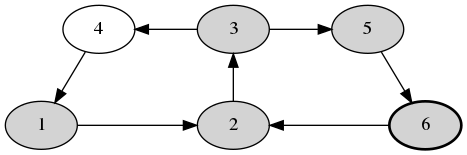
\includegraphics[width=5cm]{bstep2.png}
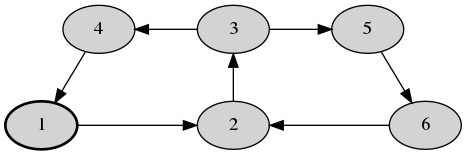
\includegraphics[width=5cm]{bstep3.png}
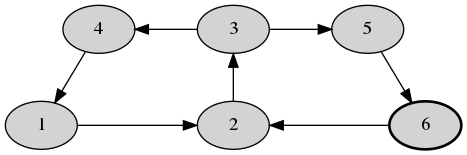
\includegraphics[width=5cm]{bstep4.png}
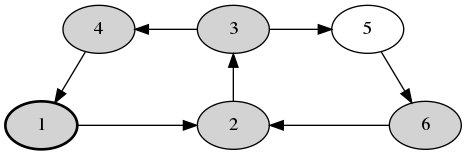
\includegraphics[width=5cm]{bstep5.png}
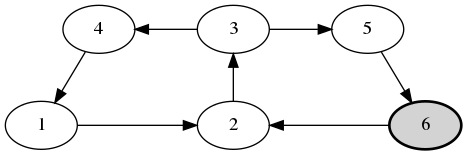
\includegraphics[width=5cm]{bstep6.png}
  \caption{Ett till exempel, med gemensamma noder på vägarna från start till slut och slut till start.}
\end{center}
\end{figure}

Det vi vill göra är alltså att hitta båda en väg från start till slut och en väg från slut till start, så att de tillsammans använder så få noder som möjligt.
I och med att dessa vägar interagerar med varandra skulle vi helst vilja konstruera dem tillsammans, en bit i taget.
Rimligtvis vill vi konstruera dem ``från vänster till höger'', med den ena vägen bakvänd, så att vi begränsar mängden interaktion --
om vi behöver minnas exakt hur vägarna vi konstruerat ser ut får vi lätt exponentiellt många tillstånd att hålla koll på, vilket inte hade fungerat.

Låt oss börja med att karaktärisera hur noderna de delar kan se ut, så att vi kan göra ovanstående mer konkret.
Tänk att det optimala svaret går från nod $1$ till nod $N$ genom noder $a_1, \dots, a_k$, och från nod $N$ till nod $1$ genom noder $b_1, \dots, b_k$.
På vilka sätt kan dessa vägar dela noder?
Rent intuitivt hade vi velat att de bara kan dela noder i motsatt ordning, så att ``vänster till höger'' blir något väldefinierat.

Låt oss tänka oss att nod $x$ och $y$ båda förekommer i både $a$ och $b$ i samma ordning.
I så fall kan vi ju minimera mängden noder i unionen av vägarna genom att låta vägen däremellan vara samma i $a$ och $b$.
I annat fall kommer noder att förekomma noder i omvänd ordning i $a$ och $b$, precis som vi hoppats.

Strukturen för en lösning ser därmed ut som i \ref{fig:lampstrukt} -- en massa gemensamma delsegment som kopplas ihop med vägar i olika riktningar.

\begin{figure}[!h]
\begin{center}
  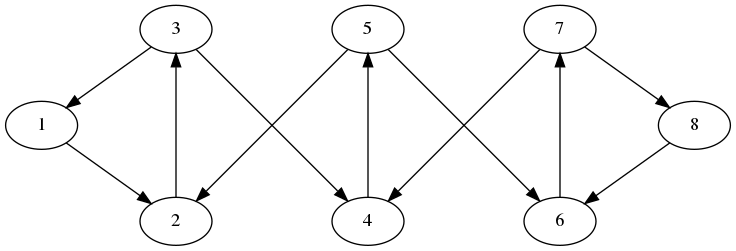
\includegraphics[width=10cm]{lampstrukt.png}
  \caption{Strukturen för en lösning. Varje kant kan ersättas av en väg med godtyckligt många noder.}
  \label{fig:lampstrukt}
\end{center}
\end{figure}

Vi kan nu återvända till vår tänkta lösning, där vi försöker konstruera de två vägarna från vänster till höger.
% Låt $E$ beteckna kanterna i graferna, och $E'$ kanterna i den omvända grafen (där alla kanter har bytt riktning).
Låt säga att vårt nuvarande tillstånd i konstruktionen av de två vägarna hela tiden är två noder $(u, v)$, rummen vi befinner oss i i framåt- och i bakåtvägarna.
Baserat på strukturen vi kommit fram till kan vi tänka oss att vi kan utföra tre olika möjliga operationer:
\begin{enumerate}
  \item Flytta $u$ framåt i grafen, till en granne.
  \item Flytta $v$ bakåt i grafen, till en granne i den reverserade grafen.
  \item Byt plats på $u$ och $v$.
\end{enumerate}

Den tredje operationen motsvarar att $u$ befinner sig i början av en delad väg och $v$ i slutet av den, och att $u$ rör sig framåt över vägen medan $v$ rör sig bakåt.

Fördelen med att vi konstruerar vägarna på sättet vi gör är att vi nu kan tilldela kostnader till de olika operationerna enbart baserat på vad $u$ och $v$ är, utan att behöva minnas hur vi flyttat oss tidigare.
Specifikt kan vi tänka att en operation av typ 1 kostar $0$ om $u$ flyttas till samma nod som $v$, annars $1$, och motsvarande för operationer av typ 2.
För operationer av typ 3 får vi en kostnad som motsvarar avståndet från nod $u$ till nod $v$ i grafen, minus $1$, i och med att noderna som är på vägen mellan $u$ och $v$ besöks exakt en gång vardera.
Se \ref{fig:lampexempel} för en illustration av hur lösningen för det andra exemplet kan beskrivas med hjälp av dessa operationer.

Givet dessa möjliga operationer och deras kostnader kan vi nu betrakta en ny graf med noder motsvarande tillstånd $(u, v)$, och kanter motsvarande operationer.
(För att beräkna kostnader för operationer av typ 3 kan vi först göra en BFS från alla noder, till kostnad $O(NE)$.)
I denna graf kan vi nu få ut vårt svar genom att göra en Dijkstra från tillstånd $(1, 1)$ till tillstånd $(N, N)$.

Antalet noder i grafen kommer att vara $O(N^2)$. Eftersom varje nods genomsnittliga antal utkanter är $2\cdot E/N + 1$ (varav $E/N$ för operationerna av typ 1 och 2, och $+ 1$ för operationen av typ 3), så kommer det totala antalet kanter att vara $O(N^2 \cdot E / N) = O(NE)$.
En Dijkstra tar därför $O(NE \log(NE))$ tid att genomföra, eller $O(NE)$ om vi utnyttjar att bara avstånd $1, 2, \dots, N-1$ är intressanta, och håller en kö för vardera av dem.
Addera till detta förberäkningen av alla kortaste avstånd som också är $O(NE)$, och vi får en total tidskomplexitet på $O(NE)$.

\begin{figure}[!h]
\begin{center}
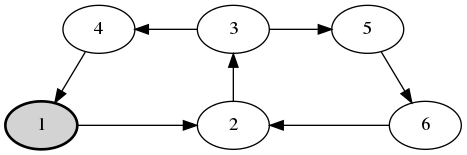
\includegraphics[width=5cm]{lampexempel1.png}
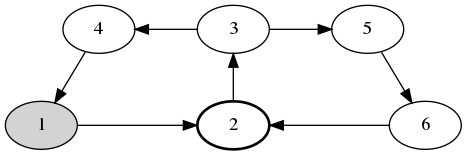
\includegraphics[width=5cm]{lampexempel2.png}
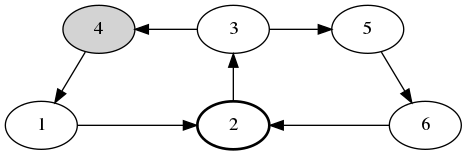
\includegraphics[width=5cm]{lampexempel3.png}
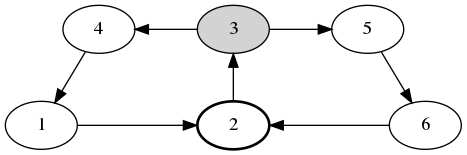
\includegraphics[width=5cm]{lampexempel4.png}
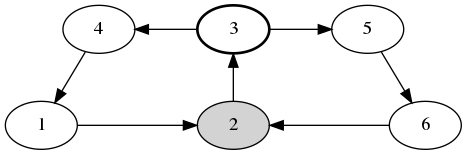
\includegraphics[width=5cm]{lampexempel5.png}
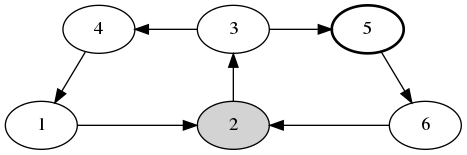
\includegraphics[width=5cm]{lampexempel6.png}
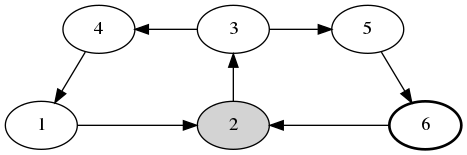
\includegraphics[width=5cm]{lampexempel7.png}
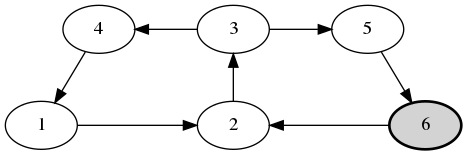
\includegraphics[width=5cm]{lampexempel8.png}
  \caption{Exempel av hur man med hjälp av operationer 1, 2 och 3 kan ta sig från tillstånd $(1,1)$ till tillstånd $(6,6)$ i grafen i det andra exemplet. $u$ betecknas med tjock ram, och $v$ med ifylld ruta.
  Stegen kostar i ordning 1, 1, 1, 0, 1, 1, 0, vilket ger en total kostnad på 5.}
  \label{fig:lampexempel}
\end{center}
\end{figure}
